\newpage
\section*{Задание 3: Редактирование изображений через Inpainting/Outpainting}
\subsection{Постановка задачи}
\noindent
Исходное изображение (Контекст): Фотография улицы с номерными знаками машин \\
Тип операции: Inpainting \\
Объект вмешательства (Промпт маски): Скрытие/Замена номера (Anonymization) \\
Сложность интеграции (Критерий качества): Естественность размытия или генерация несуществующего номера \\
Сценарий вариативности (Для аугментации): Разные форматы номеров или полная пикселизация \\
\newline
Для работы взято стоковое фото:
\begin{figure}[H]
	\centering
	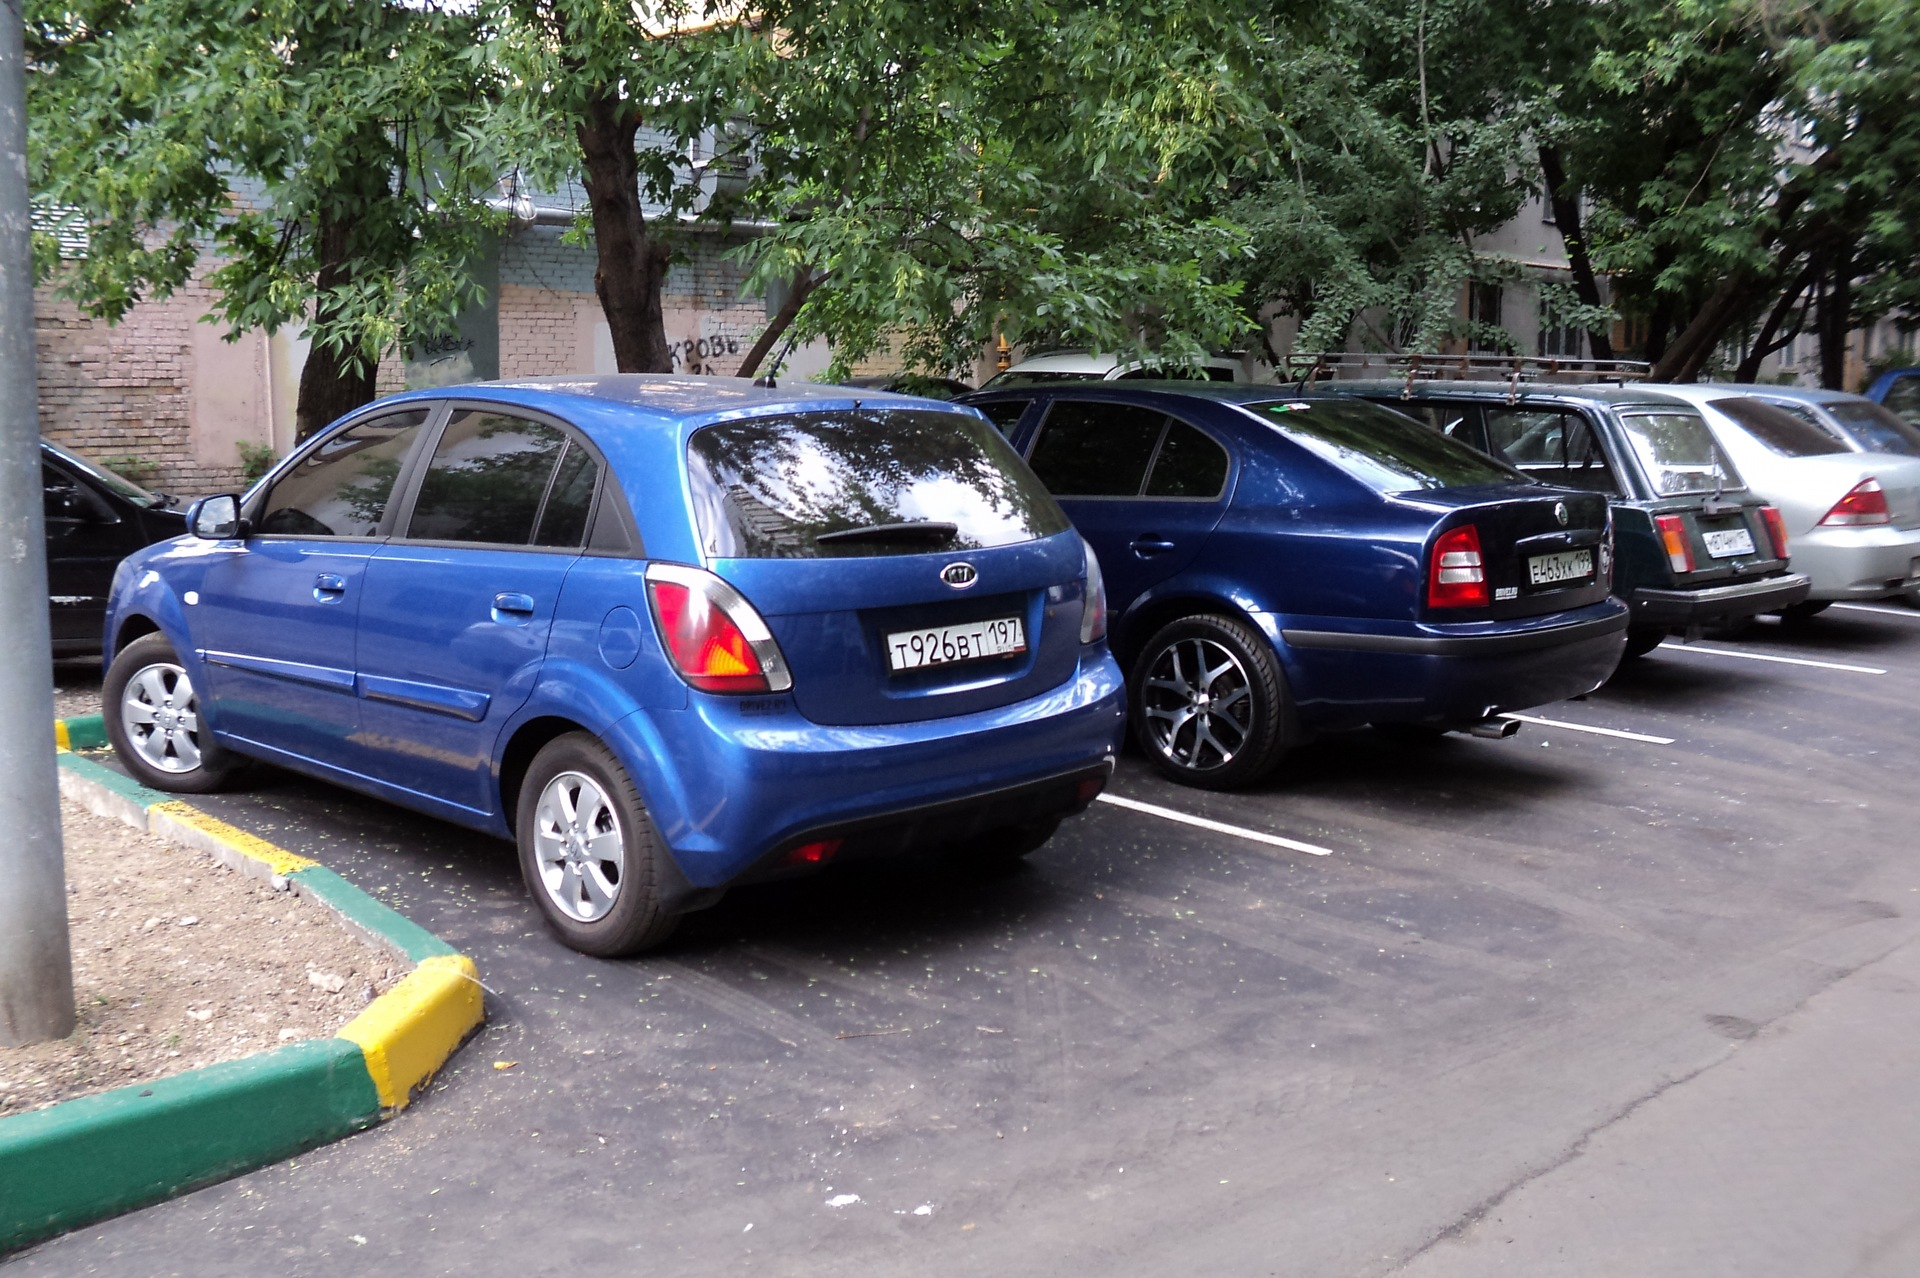
\includegraphics[width=17cm]{z3/0.jpg}
	\caption{Референс}
\end{figure}
\newpage
\subsection{Анализ контекста и планирование маски}
\noindent
Исходный контекст: \\
Освещение: солнечный день, тени падают влево-вниз.\\
Фон: городская улица, другие автомобили, тротуар.\\
Целевой объект: номерной знак (белый фон, чёрные символы, региональный код).\\
Необходимо сохранить реалистичность: тени, отражения, текстура пластика знака.\\
\newline
Выбор области маски: \\
Для inpainting выделен прямоугольник, точно покрывающий номерной знак, с небольшим захватом окружающей области (чтобы алгоритм мог учесть градиенты освещения). Маска нанесена вручную через интерфейс инструмента.
\begin{figure}[H]
	\centering
	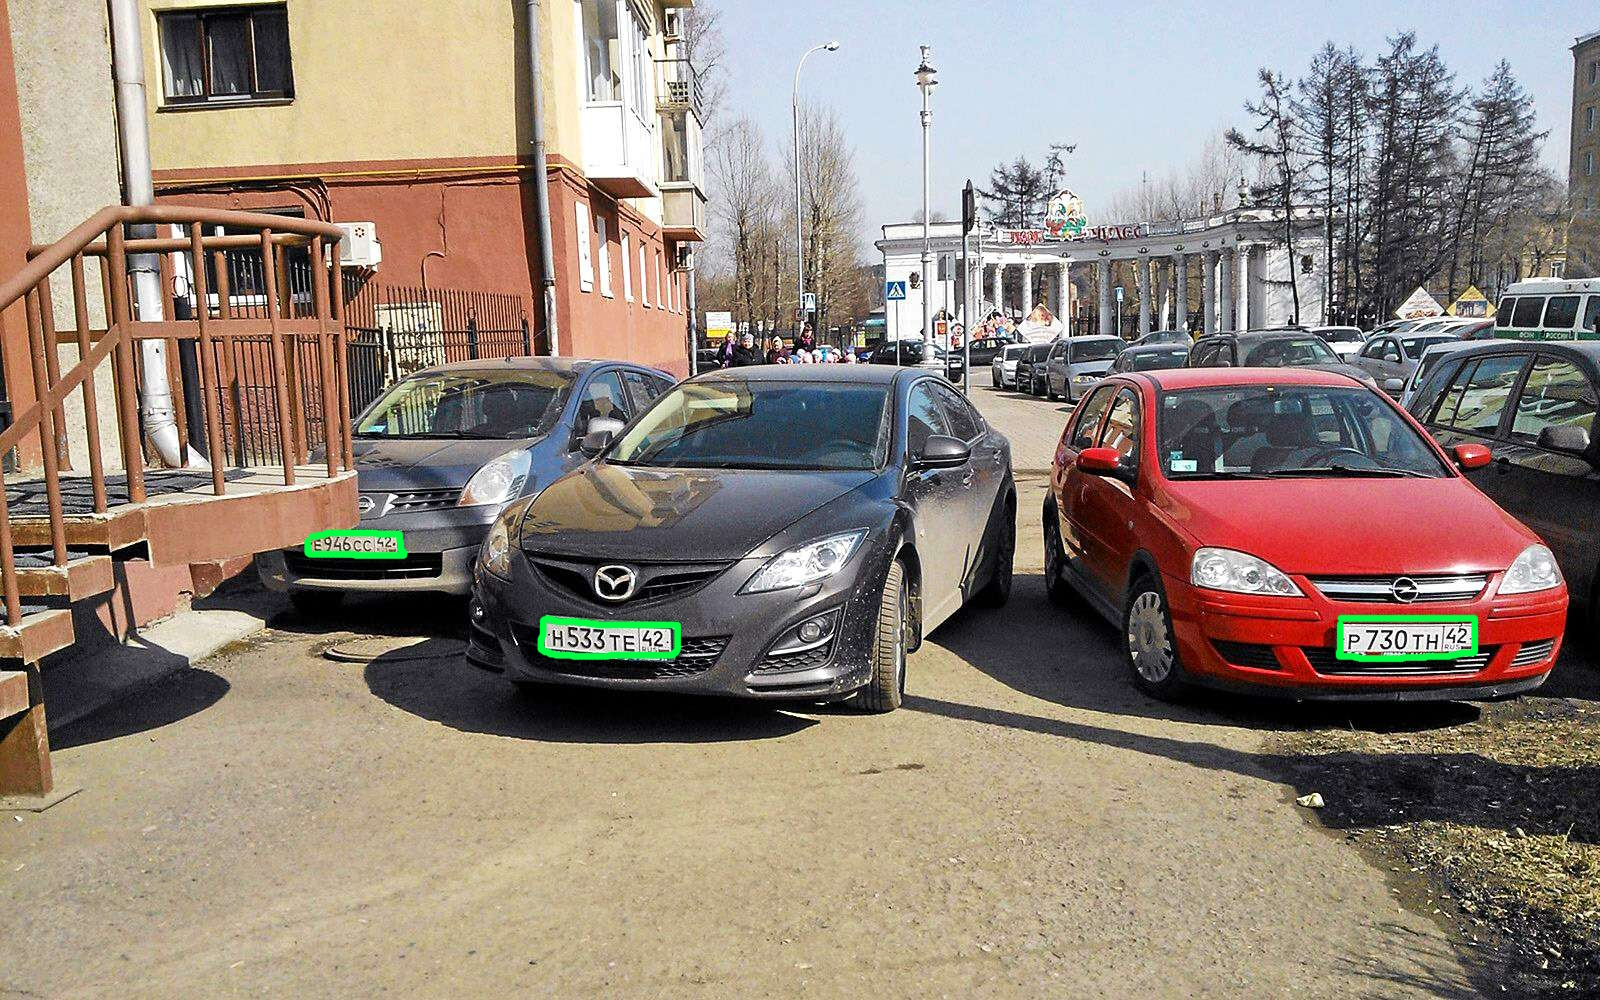
\includegraphics[width=17cm]{z3/1.jpg}
	\caption{Маска}
\end{figure}
\newpage
\subsection{Журнал генерации и отладки}
\textbf{Итерация 1: Наивный запрос} \\
Промпт v1: \textit{«Закрась номерной знак на машине, чтобы его нельзя было прочитать. Сделай это естественно, как будто знак замылен или стёрт.»} \\
\newline
Результат:
\begin{figure}[H]
	\centering
	
\includegraphics[width=17cm]{z3/1a.png}
	\caption{Итерация 1, модель (a)}
\end{figure}
Модель просто <<замылила>> номерные знаки, а также не убрала рамку на знаке у левой машины.
\newpage
\begin{figure}[H]
	\centering
	
\includegraphics[width=17cm]{z3/1b.png}
	\caption{Итерация 1, модель (b)}
\end{figure}
Модель покрыла грязью знаки так, чтобы они не читались, хоть и видно некоторые символы. \\ 
\newline
\textbf{Анализ ошибок:}
Модель интерпретировала «закрась» как изменение номера по своему усмотрению \\
\textbf{Корректировка:}
Добавить в промпт описание материала, освещения, использовать слово «заменить» вместо «закрасить», уточнить характер размытия. \\
\newline
Промпт v2:
\textit{«Замени номерной знак на автомобиле на такой же по форме и цвету, но с полностью размытыми символами, чтобы номер нельзя было распознать. Сохрани реалистичную текстуру пластика, блики от солнца и тень, падающую от знака на кузов.»}
\newpage
\begin{figure}[H]
	\centering
	
\includegraphics[width=17cm]{z3/2a.png}
	\caption{Итерация 2, модель (a)}
\end{figure}
\begin{figure}[H]
	\centering
	
\includegraphics[width=17cm]{z3/2b.png}
	\caption{Итерация 2, модель (b)}
\end{figure}
\newpage
Модель наложыла размытие на знаг строго в рамке. \\
\newline
\textbf{Анализ ошибок:}
Знак всё равно остался читаемым, даже под размытием. \\
\textbf{Корректировка:}
Явно задать замену на другой корректный номер. \\
\newline
Промпт v3:
\textit{«Полностью замени номерной знак на автомобиле. Создай реалистичный знак того же региона, но с другим, несуществующим номером: буквы и цифры должны быть чёткими, но номер вымышленный. Сохрани все блики, тени и текстуру пластика, соответствующие освещению сцены.»} \\
\newline
Результат:
\begin{figure}[H]
	\centering
	
\includegraphics[width=17cm]{z3/3a.png}
	\caption{Итерация 3, модель (a)}
\end{figure}
\newpage
\begin{figure}[H]
	\centering
	
\includegraphics[width=17cm]{z3/3b.png}
	\caption{Итерация 3, модель (b)}
\end{figure}
Модель сгенерировала три случайных номера на стандартном белом фоне. Символы чёткие, знак выглядит органично, тени и блики согласованы. Однако номер выглядит слишком новым, без следов эксплуатации, что немного выделяется на фоне остальной машины. \\
\newline
\textbf{Анализ ошибок:}
Отсутствие лёгкой «старости» знака нарушает общую реалистичность.
Но задача анонимизации решена: оригинальный номер заменён на вымышленный. \\
\textbf{Корректировка:}
Добавить модификатор «лёгкие потёртости, соответствующие возрасту автомобиля» для большей реалистичности.\\
\newline
Промпт v4 (финальный):
\textit{«Замени каждый номерной знак на автомобилях. Создай реалистичный номерной знак стандартного для этого региона образца, но с полностью вымышленным номером, например "Х999ХХ" со случайными буквами и случайными цифрми. Цифры и буквы должны быть чёткими, но знак должен иметь лёгкие следы эксплуатации (мелкие царапины, неяркие загрязнения), соответствующие общему состоянию автомобиля. Сохрани все блики от солнца, падающие тени и текстуру пластика. Интегрируй знак так, чтобы он выглядел родным для этого авто.»} \\
\newline
Результат:
\begin{figure}[H]
	\centering
	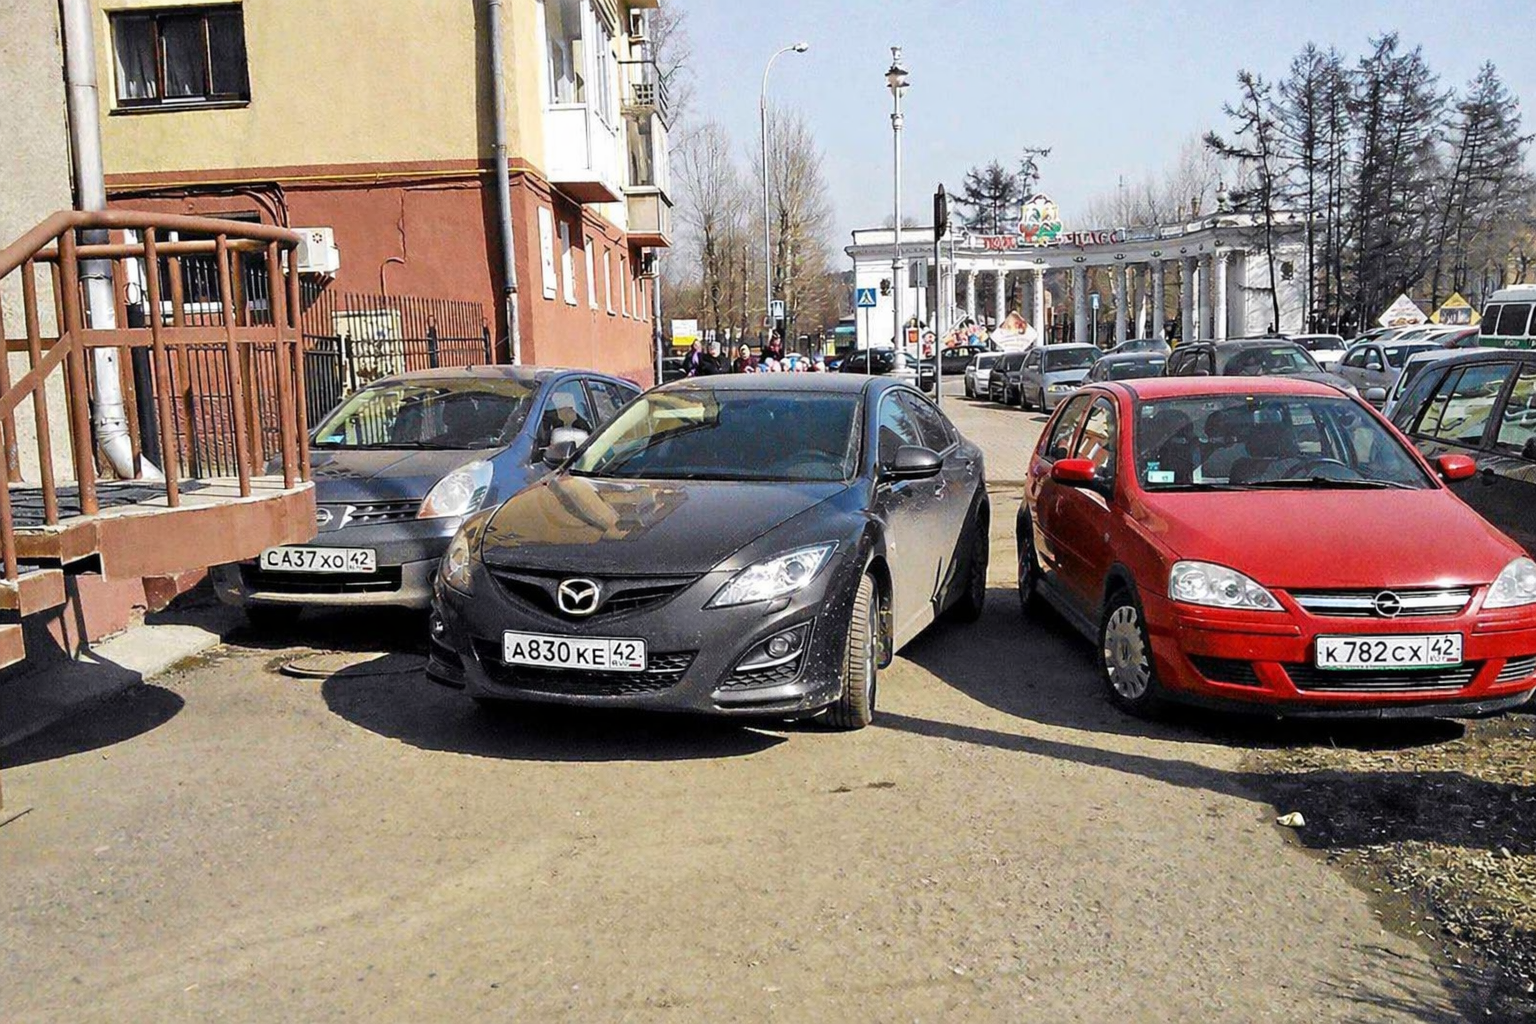
\includegraphics[width=17cm]{z3/4a.png}
	\caption{Итерация 4, модель (a)}
\end{figure}
\newpage
\begin{figure}[H]
	\centering
	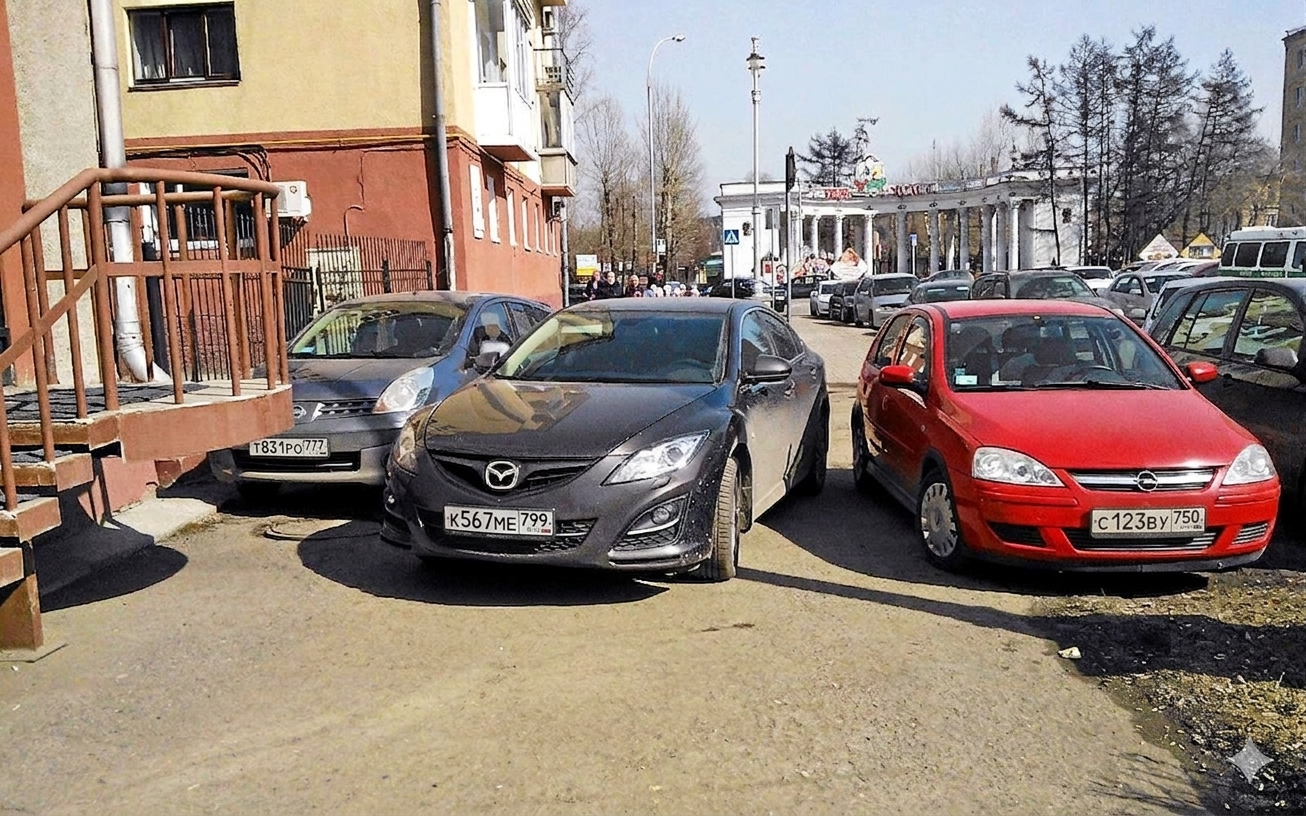
\includegraphics[width=17cm]{z3/4b.png}
	\caption{Итерация 4, модель (b)}
\end{figure}
Получены номерные знаки с вымышленными номерами «Х999ХХ», чётко читаемы, но с реалистичными потёртостями. Блики на поверхности знаков согласованы с общим освещением. Границы маски незаметны. \\
Параметры (заданы текстом): «реалистичный» – подавление артефактов. «сохрани блики, тени» – фиксация физических условий.
\subsection{Визуализация результатов}
\noindent
Исходное: Фотография улицы с тремя автомобилями	(см. рис. 16)\\
Маска: Вручную обведена вокруг знаков	зелёным цветом (см. рис. 17)\\
Итерация 1: Размытое пятно \\
Итерация 2: Размытый но читаемый знак \\
Итерация 3: Чистый знак с вымышленным номером, но слишком новый \\
Итерация 4: Реалистичные знаки «Х999ХХ» с потёртостями, согласованным освещением
\newpage
\begin{figure}[H]
	\centering
	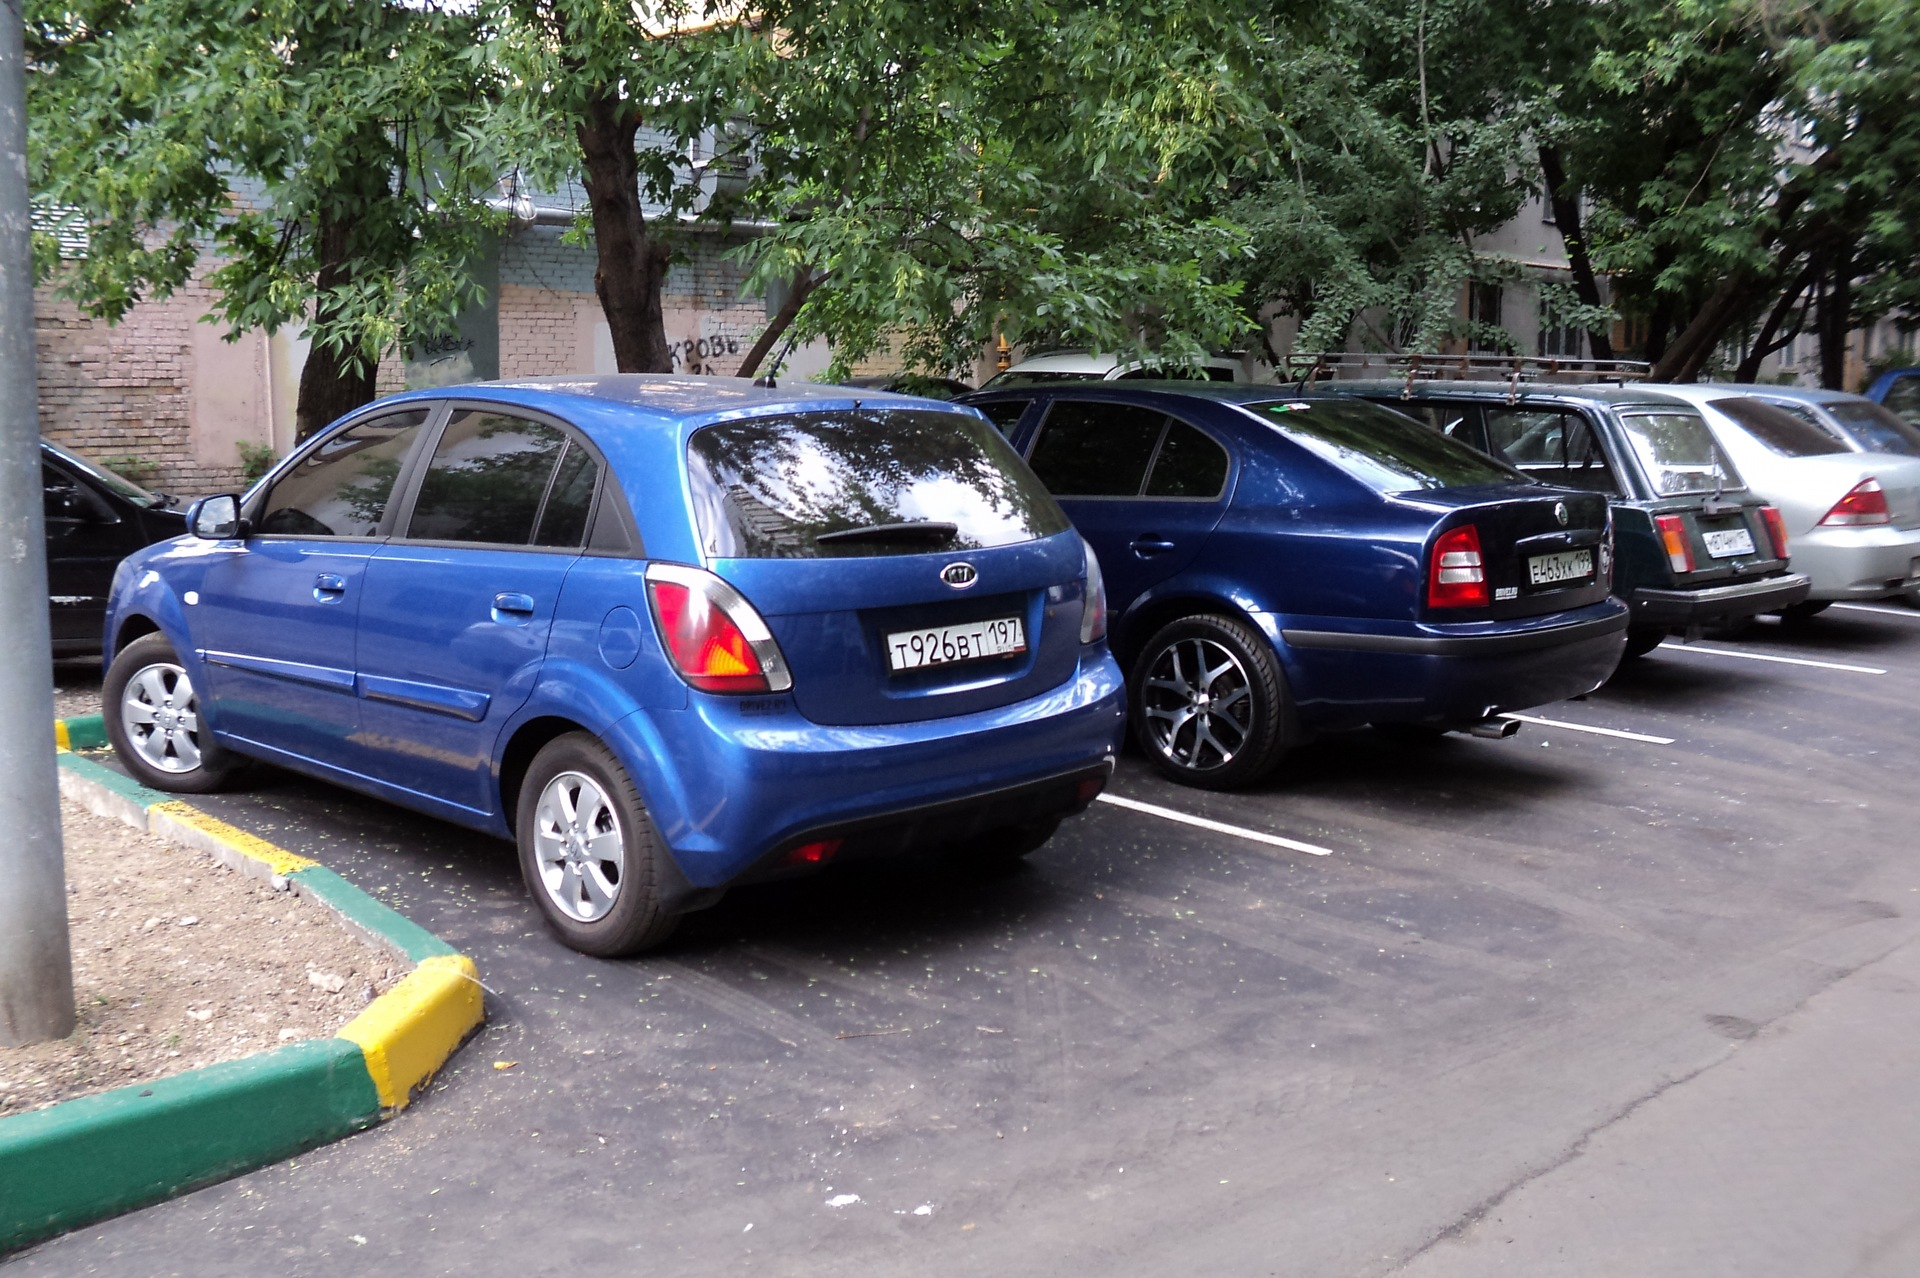
\includegraphics[width=16cm]{z3/0.jpg}
	\caption{Референс}
\end{figure}
\begin{figure}[H]
	\centering
	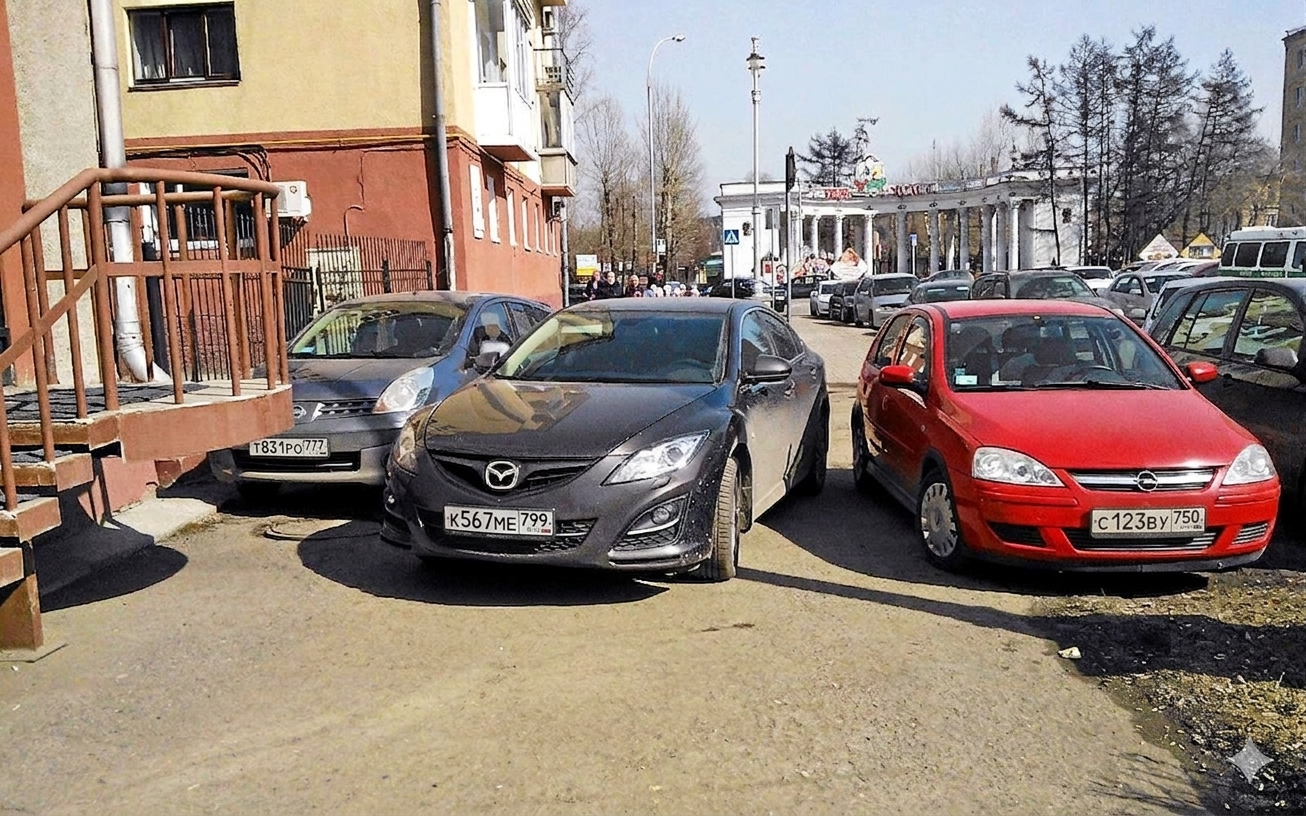
\includegraphics[width=16cm]{z3/4b.png}
	\caption{Итерация 4, модель (b)}
\end{figure}
\newpage
\subsection{Сравнение моделей}
\begin{table}[h!]
	\centering
	\begin{tabular}{|l|p{5cm}|p{5cm}|}
		\hline
		\textbf{Критерий} & \textbf{модель (a)} & \textbf{модель (b)} \\
		\hline
		Следование промпту & 5 & 5 \\
		\hline
		Качество деталей & 4 & 5 \\
		\hline
		Естественность интеграции & 0 & 5 \\
		\hline
		Вариативность  & 0 & 5 \\
		\hline
		\textbf{Итог} & 2,25 & 5\\
		\hline
	\end{tabular}
\end{table}
Модель (b) обеспечила более естественную интеграцию и точное следование инструкциям, что критически важно для анонимизации данных.
\subsection{Data Augmentation: Генерация вариаций}
Для создания набора данных (аугментации) использовался финальный промпт с заменой переменной части – самого номера.\\
\newline
Шаблон промпта:
\textit{«Замени номерной знак на автомобиле. Создай реалистичный номерной знак стандартного для этого региона образца, но с полностью вымышленным номером "\{НОМЕР\}". Цифры и буквы должны быть чёткими, но знак должен иметь лёгкие следы эксплуатации (мелкие царапины, неяркие загрязнения), соответствующие общему состоянию автомобиля. Сохрани все блики от солнца, падающие тени и текстуру пластика. Интегрируй знак так, чтобы он выглядел родным для этого авто.»} \\
\newline
Сгенерированные варианты: \\
1: А777АА \\
2: В001ВС \\
3: Е999КР \\
4: (эффект: Mosaic/Pixelate цензура) \\
\newpage
\begin{figure}[H]
	\centering
	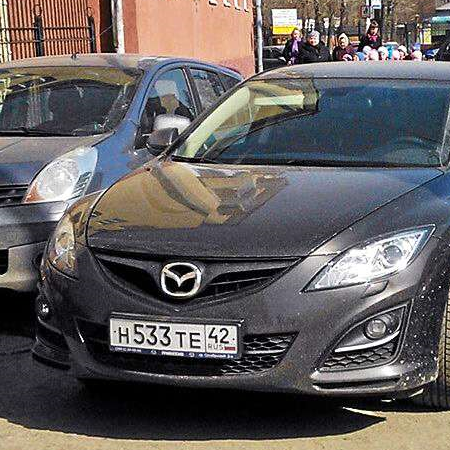
\includegraphics[width=0.45\textwidth]{z3/g0a.png}
	\hfill
	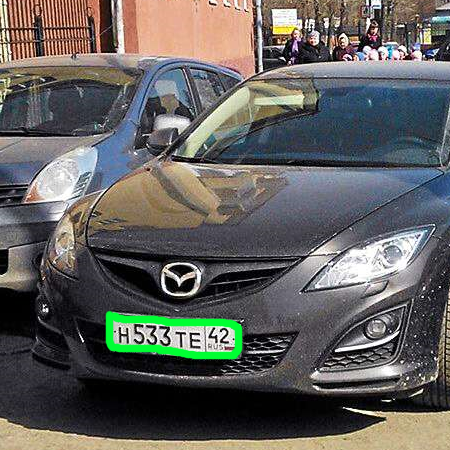
\includegraphics[width=0.45\textwidth]{z3/g0b.png}
	\caption{Референс и маска}
\end{figure}
\begin{figure}[H]
	\centering
	
\includegraphics[width=0.45\textwidth]{z3/g1.png}
	\hfill
	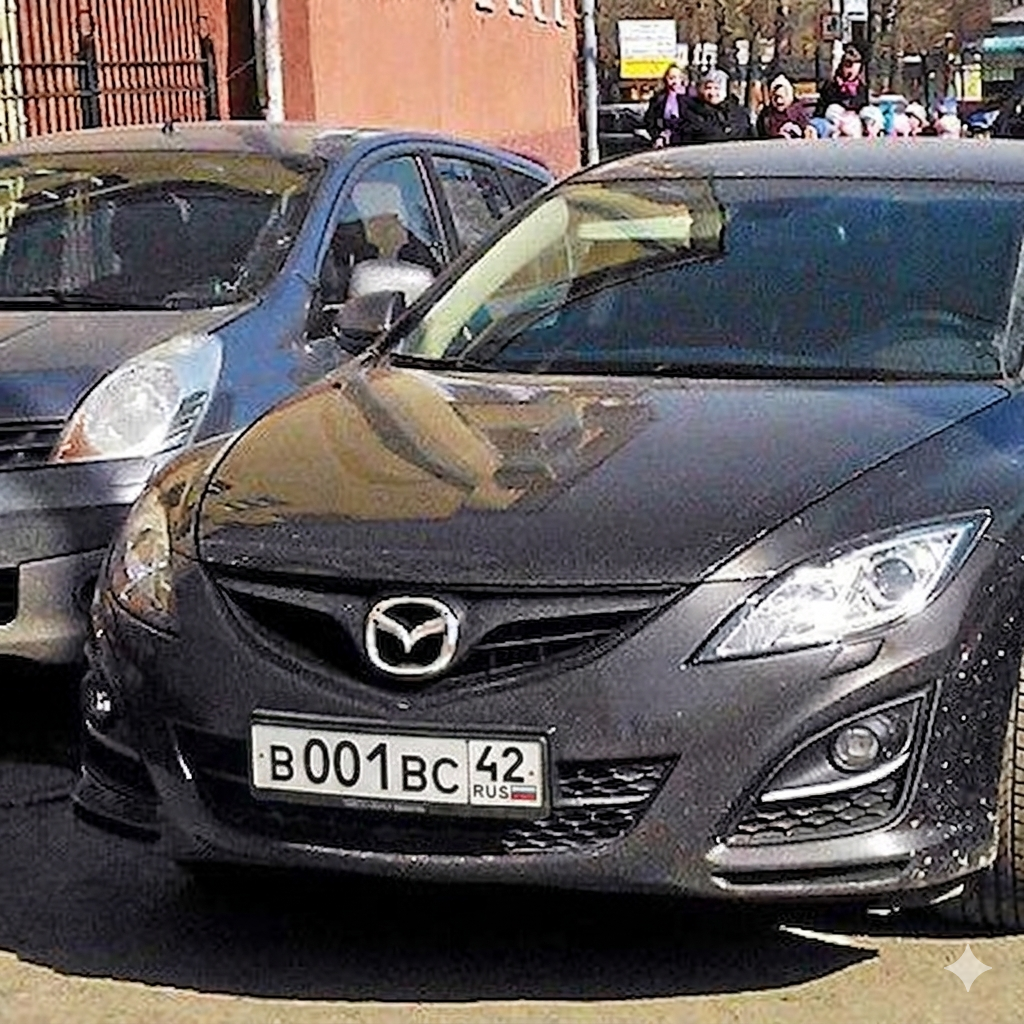
\includegraphics[width=0.45\textwidth]{z3/g2.png}
	\caption{вариант 1 и 2}
\end{figure}
\newpage
\begin{figure}[H]
	\centering
	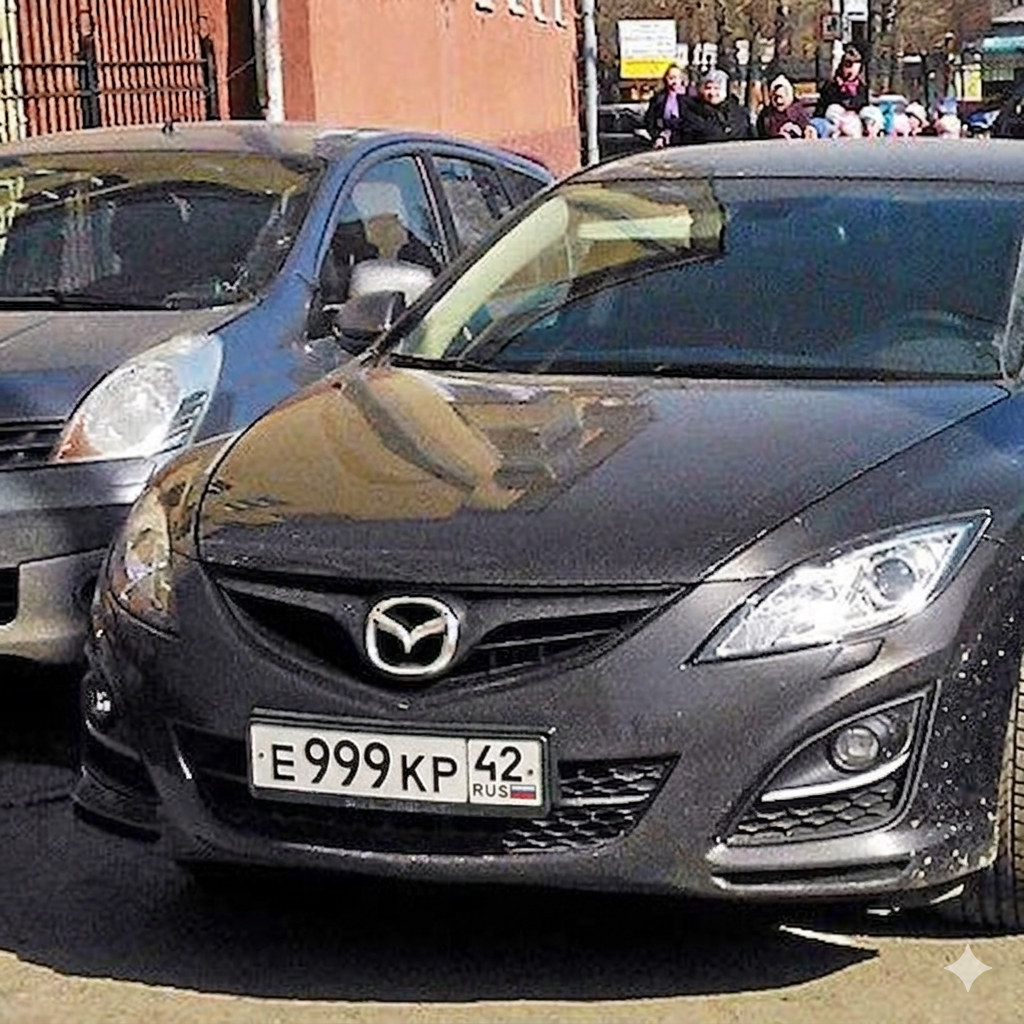
\includegraphics[width=0.45\textwidth]{z3/g3.png}
	\hfill
	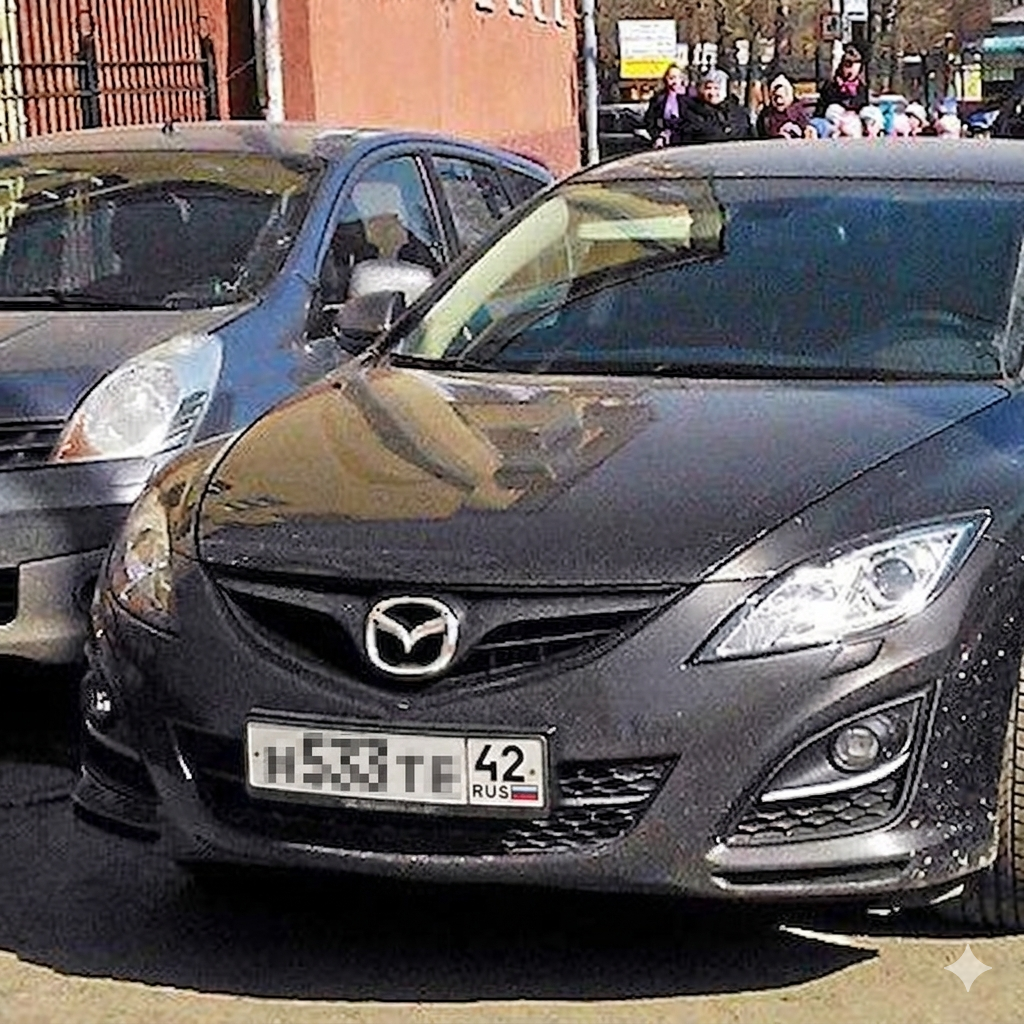
\includegraphics[width=0.45\textwidth]{z3/g4.png}
	\caption{вариант 3 и 4}
\end{figure}
\subsection{Финальный промпт}
Итоговый шаблон промпта (для inpainting):
\textit{«Замени номерной знак на автомобиле. Создай реалистичный номерной знак стандартного для этого региона образца, но с полностью вымышленным номером "\{НОМЕР\}". Цифры и буквы должны быть чёткими, но знак должен иметь лёгкие следы эксплуатации (мелкие царапины, неяркие загрязнения), соответствующие общему состоянию автомобиля. Сохрани все блики от солнца, падающие тени и текстуру пластика. Интегрируй знак так, чтобы он выглядел родным для этого авто.»} \\
\newline
Переменные части: \\
\{НОМЕР\} – подставляется желаемый номер или специальная инструкция для замены/скрытия. \\
\subsection{Вывод}
Ключевые техники, обеспечившие успех: \\
Детализация материала и освещения – описание пластика, бликов, теней заставило модель сохранить физическую согласованность. \\
Управление степенью изменений через текст – вместо параметра Denoising Strength использовались прилагательные, задающие нужную степень модификации («лёгкие следы эксплуатации» vs «эффект: Mosaic/Pixelate цензура»). \\
Итеративная отладка – последовательное уточнение от простого размытия до реалистичной замены с сохранением контекста. \\